\documentclass[10pt]{beamer}
\usepackage{hyperref}
\usepackage{fontawesome}
\usepackage{graphicx}
\usepackage[english]{babel}

% ------------------------------------------------------------------------------
% Use the beautiful metropolis beamer template
% ------------------------------------------------------------------------------
\usepackage[T1]{fontenc}
\usepackage{fontawesome}
\usepackage{FiraSans} 
\mode<presentation>
{
  \usetheme[progressbar=foot,numbering=fraction,background=light]{metropolis} 
  \usecolortheme{default} % or try albatross, beaver, crane, ...
  \usefonttheme{default}  % or try serif, structurebold, ...
  \setbeamertemplate{navigation symbols}{}
  \setbeamertemplate{caption}[numbered]
  %\setbeamertemplate{frame footer}{My custom footer}
}

% ------------------------------------------------------------------------------
% minted
% ------------------------------------------------------------------------------
\usepackage{minted}

% ------------------------------------------------------------------------------
% tikz
% ------------------------------------------------------------------------------
\usepackage{tikz}
\usetikzlibrary{calc, arrows.meta, positioning, automata}


% ------------------------------------------------------------------------------
% The Document
% ------------------------------------------------------------------------------
\title{reachability analysis for continuous one counter automata}
\author{Lars Van Roy\\
\textit{dept. of Mathematics and Computer Science} \\
\textit{University of Antwerp}\\
lars.vanroy@student.uantwerpen.be}

\begin{document}

\maketitle

\section{Current status}

\begin{frame}{Current status}
	\begin{itemize}
	    \item Continuous one counter automata
	    \begin{itemize}
	    	\pause
	    	\item No parameters
	    	\pause
	    	\item Operations: +, -
	    	\pause
	    	\item Conditions: <=, >=, =
	    \end{itemize}
	\end{itemize}
\end{frame}

\begin{frame}{Automaton}
	\begin{minipage}[t]{0.48\linewidth}
		\begin{itemize}
			\only<1->{\item Convert dot to Automaton}
			\only<2->{\item Ensure conformance
			\begin{itemize}
				\item Initial node
				\item Operations in edge
				\item Conditions in node
			\end{itemize}
			}
			\only<3->{\item Detect all loops
			\begin{itemize}
				\item Breadth first search
			\end{itemize}
			}
		\end{itemize}
	\end{minipage}
	\hfill
	\begin{minipage}[t]{0.48\linewidth}
		\only<1->{
			\begin{figure}[h!]
				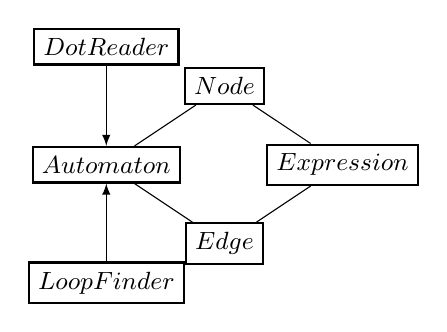
\begin{tikzpicture}[auto, >=latex, node distance = 1 cm]
					\tikzstyle{round} = [thick, draw=black, rectangle, font=\small]
					
					\node[round] 	at (0, 1.5)			(q4)	{$DotReader$};
					\node[round]	at (0, -1.5)		(q6)	{$LoopFinder$};
					
					\node[round] 	at (0, 0) 			(q0) 	{$Automaton$};
					
					\node[round] 	at (1.5, -1)	 	(q1) 	{$Edge$};
					\node[round] 	at (1.5, 1) 		(q3) 	{$Node$};
					\node[round] 	at (3, 0) 		(q5) 	{$Expression$};
					
					\path[->]
					(q6)	edge	node {$ $}	(q0)
					(q4)	edge	node {$ $}	(q0);
					
					\path[-]
					(q0)	edge	node {$ $}	(q1)
					(q0)	edge	node {$ $}	(q3)
					(q1)	edge	node {$ $}	(q5)
					(q3)	edge	node {$ $}	(q5);
				\end{tikzpicture}
			\end{figure}
		}
	\end{minipage}
\end{frame}

\begin{frame}{Initial node}
	\begin{figure}[h!]
		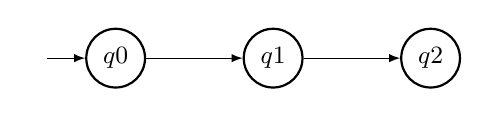
\begin{tikzpicture}[auto, >=latex, node distance = 1 cm]
		\tikzstyle{round} = [thick, draw=black, circle, font=\small]
		\tikzstyle{invis} = [draw=none, font=\small]
		
		\node[invis]			at (-1,0)		(q3)	{$ $};
		\node[round] 			at (0, 0) 		(q0) 	{$q0$};
		\node[round] 			at (2, 0) 		(q1) 	{$q1$};
		\node[round] 			at (4, 0) 		(q2) 	{$q2$};
		
		\path[->]
		(q3)	edge	node {$ $}	(q0)
		(q0)	edge	node {$ $}	(q1)
		(q1)	edge	node {$ $}	(q2);
		\end{tikzpicture}
	\end{figure}
\end{frame}

\begin{frame}{Operation in node}
	\begin{minipage}[t]{0.48\linewidth}
		\begin{itemize}
			\only<1->{\item Given a node with an operation label}
			\only<2->{\item Insert a new node}
			\only<3->{\item Create an edge to this node}
			\only<3->{\item Add the operation to the edge}
			\only<4->{\item Reconnect all pre-existing edges}
		\end{itemize}
	\end{minipage}
	\hfill
	\begin{minipage}[t]{0.48\linewidth}
		\only<1>{
			\begin{figure}[h!]
				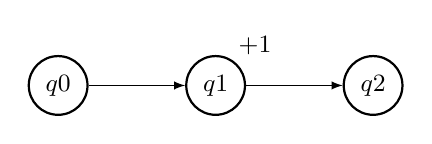
\begin{tikzpicture}[auto, >=latex, node distance = 1 cm]
				\tikzstyle{round} = [thick, draw=black, circle, font=\small]
				\tikzstyle{invis} = [draw=none, font=\small]
				
				\node[round] 	at (0, 0) 		(q0) 	{$q0$};
				\node[round] 	at (2, 0)		(q1) 	{$q1$};
				\node[invis]	at (2.5, 0.5)	(q3)	{$+1$};
				\node[round] 	at (4, 0) 		(q2) 	{$q2$};
				
				\path[->]
				(q0)	edge	node {$ $}	(q1)
				(q1)	edge	node {$ $}	(q2);
				\end{tikzpicture}
			\end{figure}
		}
		\only<2>{
			\begin{figure}[h!]
				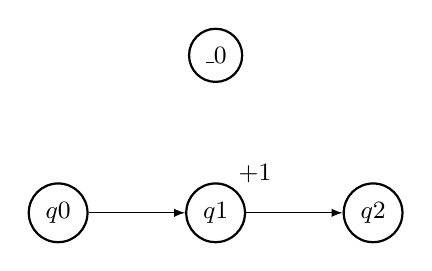
\begin{tikzpicture}[auto, >=latex, node distance = 1 cm]
				\tikzstyle{round} = [thick, draw=black, circle, font=\small]
				\tikzstyle{invis} = [draw=none, font=\small]
				
				\node[round] 	at (0, 0) 		(q0) 	{$q0$};
				\node[round] 	at (2, 0)		(q1) 	{$q1$};
				\node[invis]	at (2.5, 0.5)	(q3)	{$+1$};
				\node[round] 	at (4, 0) 		(q2) 	{$q2$};
				\node[round] 	at (2, 2) 		(q4) 	{$\_0$};
				
				\path[->]
				(q0)	edge	node {$ $}	(q1)
				(q1)	edge	node {$ $}	(q2);
				\end{tikzpicture}
			\end{figure}
		}
		\only<3>{
			\begin{figure}[h!]
				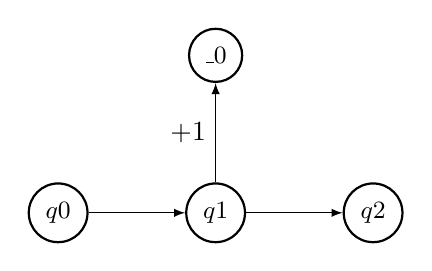
\begin{tikzpicture}[auto, >=latex, node distance = 1 cm]
				\tikzstyle{round} = [thick, draw=black, circle, font=\small]
				\tikzstyle{invis} = [draw=none, font=\small]
				
				\node[round] 	at (0, 0) 		(q0) 	{$q0$};
				\node[round] 	at (2, 0)		(q1) 	{$q1$};
				\node[round] 	at (4, 0) 		(q2) 	{$q2$};
				\node[round] 	at (2, 2) 		(q4) 	{$\_0$};
				
				\path[->]
				(q0)	edge	node {$ $}	(q1)
				(q1)	edge	node {$ $}	(q2)
				(q1)	edge	node {$+1$}	(q4);
				\end{tikzpicture}
			\end{figure}
		}
		\only<4>{
			\begin{figure}[h!]
				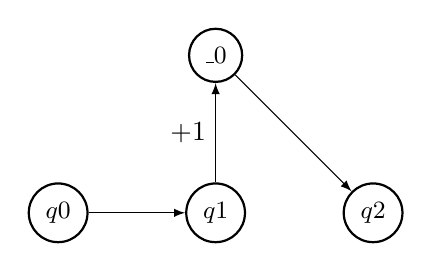
\begin{tikzpicture}[auto, >=latex, node distance = 1 cm]
				\tikzstyle{round} = [thick, draw=black, circle, font=\small]
				\tikzstyle{invis} = [draw=none, font=\small]
				
				\node[round] 	at (0, 0) 		(q0) 	{$q0$};
				\node[round] 	at (2, 0)		(q1) 	{$q1$};
				\node[round] 	at (4, 0) 		(q2) 	{$q2$};
				\node[round] 	at (2, 2) 		(q4) 	{$\_0$};
				
				\path[->]
				(q0)	edge	node {$ $}	(q1)
				(q4)	edge	node {$ $}	(q2)
				(q1)	edge	node {$+1$}	(q4);
				\end{tikzpicture}
			\end{figure}
		}
	\end{minipage}
\end{frame}

\begin{frame}{Condition in edge}
	\begin{minipage}[t]{0.48\linewidth}
		\begin{itemize}
			\only<1->{\item Given an edge with a conditional label}
			\only<2->{\item Insert a new node}
			\only<2->{\item Add the condition to the node}
			\only<3->{\item Connect the two nodes via the new node}
			\only<4->{\item Remove the old edge}
		\end{itemize}
	\end{minipage}
	\hfill
	\begin{minipage}[t]{0.48\linewidth}
		\only<1>{
			\begin{figure}[h!]
				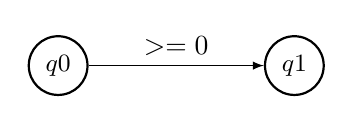
\begin{tikzpicture}[auto, >=latex, node distance = 1 cm]
				\tikzstyle{round} = [thick, draw=black, circle, font=\small]
				\tikzstyle{invis} = [draw=none, font=\small]
				
				\node[round] 	at (0, 0) 		(q0) 	{$q0$};
				\node[round] 	at (3, 0)		(q1) 	{$q1$};
				
				\path[->]
				(q0)	edge	node {$>= 0$}	(q1);
				\end{tikzpicture}
			\end{figure}
		}
		\only<2>{
			\begin{figure}[h!]
				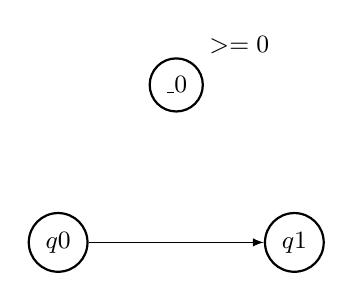
\begin{tikzpicture}[auto, >=latex, node distance = 1 cm]
				\tikzstyle{round} = [thick, draw=black, circle, font=\small]
				\tikzstyle{invis} = [draw=none, font=\small]
				
				\node[round] 	at (0, 0) 		(q0) 	{$q0$};
				\node[round] 	at (3, 0)		(q1) 	{$q1$};
				\node[invis]	at (2.3, 2.5)		(q3)	{$>=0$};
				\node[round] 	at (1.5, 2) 	(q4) 	{$\_0$};
				
				\path[->]
				(q0)	edge	node {$ $}	(q1);
				\end{tikzpicture}
			\end{figure}
		}
		\only<3>{
			\begin{figure}[h!]
				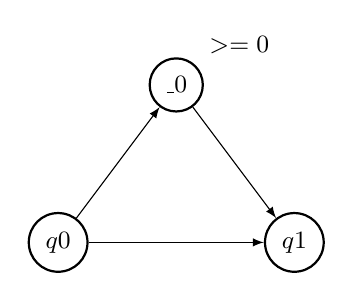
\begin{tikzpicture}[auto, >=latex, node distance = 1 cm]
				\tikzstyle{round} = [thick, draw=black, circle, font=\small]
				\tikzstyle{invis} = [draw=none, font=\small]
				
				\node[round] 	at (0, 0) 		(q0) 	{$q0$};
				\node[round] 	at (3, 0)		(q1) 	{$q1$};
				\node[invis]	at (2.3, 2.5)		(q3)	{$>=0$};
				\node[round] 	at (1.5, 2) 	(q4) 	{$\_0$};
				
				\path[->]
				(q0)	edge	node {$ $}	(q1)
				(q0)	edge	node {$ $}	(q4)
				(q4)	edge	node {$ $}	(q1);
				\end{tikzpicture}
			\end{figure}
		}
		\only<4>{
			\begin{figure}[h!]
				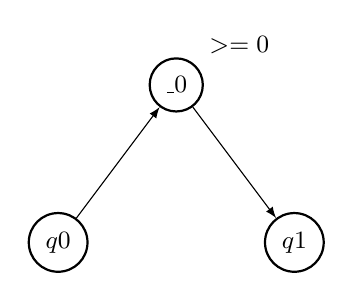
\begin{tikzpicture}[auto, >=latex, node distance = 1 cm]
				\tikzstyle{round} = [thick, draw=black, circle, font=\small]
				\tikzstyle{invis} = [draw=none, font=\small]
				
				\node[round] 	at (0, 0) 		(q0) 	{$q0$};
				\node[round] 	at (3, 0)		(q1) 	{$q1$};
				\node[invis]	at (2.3, 2.5)		(q3)	{$>=0$};
				\node[round] 	at (1.5, 2) 	(q4) 	{$\_0$};
				
				\path[->]
				(q0)	edge	node {$ $}	(q4)
				(q4)	edge	node {$ $}	(q1);
				\end{tikzpicture}
			\end{figure}
		}
	\end{minipage}
\end{frame}

\begin{frame}{Reachability}
	\begin{minipage}[t]{0.48\linewidth}
		\begin{itemize}
			\only<1->{\item Initialise Reach per node}
			\only<2->{
				\item Update Reach instances
				\begin{itemize}
					\item Do one update step
					\item Rescale Reach
					\item Check loop acceleration
					\item Check end condition
				\end{itemize}
			}
			\only<3->{
				\item Reachability
				\begin{itemize}
					\item Node has a Reach that is not empty
				\end{itemize}
			}
		\end{itemize}
	\end{minipage}
	\hfill
	\begin{minipage}[t]{0.48\linewidth}
		\begin{figure}[h!]
			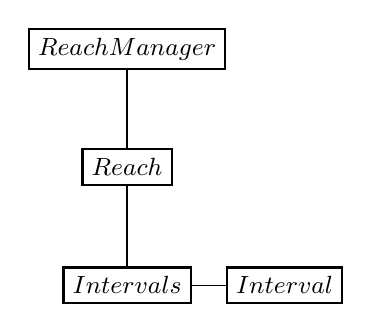
\begin{tikzpicture}[auto, >=latex, node distance = 1 cm]
			\tikzstyle{round} = [thick, draw=black, rectangle, font=\small]
			
			\node[round] 	at (0, 1.5) 		(q0) 	{$ReachManager$};
			\node[round]	at (0, 0)			(q1)	{$Reach$};
			\node[round] 	at (0, -1.5)		(q2)	{$Intervals$};
			\node[round] 	at (2, -1.5) 	(q3) 	{$Interval$};
			
			\path[-]
			(q0)	edge	node {$ $}	(q1)
			(q1)	edge	node {$ $}	(q2)
			(q2)	edge	node {$ $}	(q3);
			\end{tikzpicture}
		\end{figure}
	\end{minipage}
\end{frame}

\begin{frame}{Remaining work}
	\begin{itemize}
		\item Add support for parametric counter automata
		\pause
		\item Apply to a (or more) bigger use case(s)
		\item Document the results
	\end{itemize}
\end{frame}

\end{document}
